\documentclass[11pt]{article}
    \usepackage[breakable]{tcolorbox}
    \usepackage{parskip} % Stop auto-indenting (to mimic markdown behaviour)
    

    % Basic figure setup, for now with no caption control since it's done
    % automatically by Pandoc (which extracts ![](path) syntax from Markdown).
    \usepackage{graphicx}
    % Keep aspect ratio if custom image width or height is specified
    \setkeys{Gin}{keepaspectratio}
    % Maintain compatibility with old templates. Remove in nbconvert 6.0
    \let\Oldincludegraphics\includegraphics
    % Ensure that by default, figures have no caption (until we provide a
    % proper Figure object with a Caption API and a way to capture that
    % in the conversion process - todo).
    \usepackage{caption}
    \DeclareCaptionFormat{nocaption}{}
    \captionsetup{format=nocaption,aboveskip=0pt,belowskip=0pt}

    \usepackage{float}
    \floatplacement{figure}{H} % forces figures to be placed at the correct location
    \usepackage{xcolor} % Allow colors to be defined
    \usepackage{enumerate} % Needed for markdown enumerations to work
    \usepackage{geometry} % Used to adjust the document margins
    \usepackage{amsmath} % Equations
    \usepackage{amssymb} % Equations
    \usepackage{textcomp} % defines textquotesingle
    % Hack from http://tex.stackexchange.com/a/47451/13684:
    \AtBeginDocument{%
        \def\PYZsq{\textquotesingle}% Upright quotes in Pygmentized code
    }
    \usepackage{upquote} % Upright quotes for verbatim code
    \usepackage{eurosym} % defines \euro

    \usepackage{iftex}
    \ifPDFTeX
        \usepackage[T1]{fontenc}
        \IfFileExists{alphabeta.sty}{
              \usepackage{alphabeta}
          }{
              \usepackage[mathletters]{ucs}
              \usepackage[utf8x]{inputenc}
          }
    \else
        \usepackage{fontspec}
        \usepackage{unicode-math}
    \fi

    \usepackage{fancyvrb} % verbatim replacement that allows latex
    \usepackage{grffile} % extends the file name processing of package graphics
 	                        % to support a larger range
    \usetikzlibrary{positioning, arrows}
    \makeatletter % fix for old versions of grffile with XeLaTeX
    \@ifpackagelater{grffile}{2019/11/01}
    {
      % Do nothing on new versions
    }
    {
      \def\Gread@@xetex#1{%
        \IfFileExists{"\Gin@base".bb}%
        {\Gread@eps{\Gin@base.bb}}%
        {\Gread@@xetex@aux#1}%
      }
    }
    \makeatother
    \usepackage[Export]{adjustbox} % Used to constrain images to a maximum size
    \adjustboxset{max size={0.9\linewidth}{0.9\paperheight}}

    % The hyperref package gives us a pdf with properly built
    % internal navigation ('pdf bookmarks' for the table of contents,
    % internal cross-reference links, web links for URLs, etc.)
    \usepackage{hyperref}
    % The default LaTeX title has an obnoxious amount of whitespace. By default,
    % titling removes some of it. It also provides customization options.
    \usepackage{titling}
    \usepackage{longtable} % longtable support required by pandoc >1.10
    \usepackage{booktabs}  % table support for pandoc > 1.12.2
    \usepackage{array}     % table support for pandoc >= 2.11.3
    \usepackage{calc}      % table minipage width calculation for pandoc >= 2.11.1
    \usepackage[inline]{enumitem} % IRkernel/repr support (it uses the enumerate* environment)
    \usepackage[normalem]{ulem} % ulem is needed to support strikethroughs (\sout)
                                % normalem makes italics be italics, not underlines
    \usepackage{soul}      % strikethrough (\st) support for pandoc >= 3.0.0
    \usepackage{mathrsfs}
    

    
    % Colors for the hyperref package
    \definecolor{urlcolor}{rgb}{0,.145,.698}
    \definecolor{linkcolor}{rgb}{.71,0.21,0.01}
    \definecolor{citecolor}{rgb}{.12,.54,.11}

    % ANSI colors
    \definecolor{ansi-black}{HTML}{3E424D}
    \definecolor{ansi-black-intense}{HTML}{282C36}
    \definecolor{ansi-red}{HTML}{E75C58}
    \definecolor{ansi-red-intense}{HTML}{B22B31}
    \definecolor{ansi-green}{HTML}{00A250}
    \definecolor{ansi-green-intense}{HTML}{007427}
    \definecolor{ansi-yellow}{HTML}{DDB62B}
    \definecolor{ansi-yellow-intense}{HTML}{B27D12}
    \definecolor{ansi-blue}{HTML}{208FFB}
    \definecolor{ansi-blue-intense}{HTML}{0065CA}
    \definecolor{ansi-magenta}{HTML}{D160C4}
    \definecolor{ansi-magenta-intense}{HTML}{A03196}
    \definecolor{ansi-cyan}{HTML}{60C6C8}
    \definecolor{ansi-cyan-intense}{HTML}{258F8F}
    \definecolor{ansi-white}{HTML}{C5C1B4}
    \definecolor{ansi-white-intense}{HTML}{A1A6B2}
    \definecolor{ansi-default-inverse-fg}{HTML}{FFFFFF}
    \definecolor{ansi-default-inverse-bg}{HTML}{000000}

    % common color for the border for error outputs.
    \definecolor{outerrorbackground}{HTML}{FFDFDF}

    % commands and environments needed by pandoc snippets
    % extracted from the output of `pandoc -s`
    \providecommand{\tightlist}{%
      \setlength{\itemsep}{0pt}\setlength{\parskip}{0pt}}
    \DefineVerbatimEnvironment{Highlighting}{Verbatim}{commandchars=\\\{\}}
    % Add ',fontsize=\small' for more characters per line
    \newenvironment{Shaded}{}{}
    \newcommand{\KeywordTok}[1]{\textcolor[rgb]{0.00,0.44,0.13}{\textbf{{#1}}}}
    \newcommand{\DataTypeTok}[1]{\textcolor[rgb]{0.56,0.13,0.00}{{#1}}}
    \newcommand{\DecValTok}[1]{\textcolor[rgb]{0.25,0.63,0.44}{{#1}}}
    \newcommand{\BaseNTok}[1]{\textcolor[rgb]{0.25,0.63,0.44}{{#1}}}
    \newcommand{\FloatTok}[1]{\textcolor[rgb]{0.25,0.63,0.44}{{#1}}}
    \newcommand{\CharTok}[1]{\textcolor[rgb]{0.25,0.44,0.63}{{#1}}}
    \newcommand{\StringTok}[1]{\textcolor[rgb]{0.25,0.44,0.63}{{#1}}}
    \newcommand{\CommentTok}[1]{\textcolor[rgb]{0.38,0.63,0.69}{\textit{{#1}}}}
    \newcommand{\OtherTok}[1]{\textcolor[rgb]{0.00,0.44,0.13}{{#1}}}
    \newcommand{\AlertTok}[1]{\textcolor[rgb]{1.00,0.00,0.00}{\textbf{{#1}}}}
    \newcommand{\FunctionTok}[1]{\textcolor[rgb]{0.02,0.16,0.49}{{#1}}}
    \newcommand{\RegionMarkerTok}[1]{{#1}}
    \newcommand{\ErrorTok}[1]{\textcolor[rgb]{1.00,0.00,0.00}{\textbf{{#1}}}}
    \newcommand{\NormalTok}[1]{{#1}}

    % Additional commands for more recent versions of Pandoc
    \newcommand{\ConstantTok}[1]{\textcolor[rgb]{0.53,0.00,0.00}{{#1}}}
    \newcommand{\SpecialCharTok}[1]{\textcolor[rgb]{0.25,0.44,0.63}{{#1}}}
    \newcommand{\VerbatimStringTok}[1]{\textcolor[rgb]{0.25,0.44,0.63}{{#1}}}
    \newcommand{\SpecialStringTok}[1]{\textcolor[rgb]{0.73,0.40,0.53}{{#1}}}
    \newcommand{\ImportTok}[1]{{#1}}
    \newcommand{\DocumentationTok}[1]{\textcolor[rgb]{0.73,0.13,0.13}{\textit{{#1}}}}
    \newcommand{\AnnotationTok}[1]{\textcolor[rgb]{0.38,0.63,0.69}{\textbf{\textit{{#1}}}}}
    \newcommand{\CommentVarTok}[1]{\textcolor[rgb]{0.38,0.63,0.69}{\textbf{\textit{{#1}}}}}
    \newcommand{\VariableTok}[1]{\textcolor[rgb]{0.10,0.09,0.49}{{#1}}}
    \newcommand{\ControlFlowTok}[1]{\textcolor[rgb]{0.00,0.44,0.13}{\textbf{{#1}}}}
    \newcommand{\OperatorTok}[1]{\textcolor[rgb]{0.40,0.40,0.40}{{#1}}}
    \newcommand{\BuiltInTok}[1]{{#1}}
    \newcommand{\ExtensionTok}[1]{{#1}}
    \newcommand{\PreprocessorTok}[1]{\textcolor[rgb]{0.74,0.48,0.00}{{#1}}}
    \newcommand{\AttributeTok}[1]{\textcolor[rgb]{0.49,0.56,0.16}{{#1}}}
    \newcommand{\InformationTok}[1]{\textcolor[rgb]{0.38,0.63,0.69}{\textbf{\textit{{#1}}}}}
    \newcommand{\WarningTok}[1]{\textcolor[rgb]{0.38,0.63,0.69}{\textbf{\textit{{#1}}}}}

\DeclareMathOperator{\Lap}{\mathcal{L}}
\DeclareMathOperator{\Var}{Var} % varience
\DeclareMathOperator{\Cov}{Cov} % covarience
\DeclareMathOperator{\E}{E} % expected
\DeclareMathOperator{\Bern}{Bern}
\DeclareMathOperator{\Binom}{Binom}
\DeclareMathOperator{\Poisson}{Poisson}

    \makeatletter
    \newsavebox\pandoc@box
    \newcommand*\pandocbounded[1]{%
      \sbox\pandoc@box{#1}%
      % scaling factors for width and height
      \Gscale@div\@tempa\textheight{\dimexpr\ht\pandoc@box+\dp\pandoc@box\relax}%
      \Gscale@div\@tempb\linewidth{\wd\pandoc@box}%
      % select the smaller of both
      \ifdim\@tempb\p@<\@tempa\p@
        \let\@tempa\@tempb
      \fi
      % scaling accordingly (\@tempa < 1)
      \ifdim\@tempa\p@<\p@
        \scalebox{\@tempa}{\usebox\pandoc@box}%
      % scaling not needed, use as it is
      \else
        \usebox{\pandoc@box}%
      \fi
    }
    \makeatother

    % Define a nice break command that doesn't care if a line doesn't already
    % exist.
    \def\br{\hspace*{\fill} \\* }
    % Math Jax compatibility definitions
    \def\gt{>}
    \def\lt{<}
    \let\Oldtex\TeX
    \let\Oldlatex\LaTeX
    \renewcommand{\TeX}{\textrm{\Oldtex}}
    \renewcommand{\LaTeX}{\textrm{\Oldlatex}}
    % Document parameters
    % Document title
    \title{Homework\_06}
    
    
    
    
    
    
    
% Pygments definitions
\makeatletter
\def\PY@reset{\let\PY@it=\relax \let\PY@bf=\relax%
    \let\PY@ul=\relax \let\PY@tc=\relax%
    \let\PY@bc=\relax \let\PY@ff=\relax}
\def\PY@tok#1{\csname PY@tok@#1\endcsname}
\def\PY@toks#1+{\ifx\relax#1\empty\else%
    \PY@tok{#1}\expandafter\PY@toks\fi}
\def\PY@do#1{\PY@bc{\PY@tc{\PY@ul{%
    \PY@it{\PY@bf{\PY@ff{#1}}}}}}}
\def\PY#1#2{\PY@reset\PY@toks#1+\relax+\PY@do{#2}}

\@namedef{PY@tok@w}{\def\PY@tc##1{\textcolor[rgb]{0.73,0.73,0.73}{##1}}}
\@namedef{PY@tok@c}{\let\PY@it=\textit\def\PY@tc##1{\textcolor[rgb]{0.24,0.48,0.48}{##1}}}
\@namedef{PY@tok@cp}{\def\PY@tc##1{\textcolor[rgb]{0.61,0.40,0.00}{##1}}}
\@namedef{PY@tok@k}{\let\PY@bf=\textbf\def\PY@tc##1{\textcolor[rgb]{0.00,0.50,0.00}{##1}}}
\@namedef{PY@tok@kp}{\def\PY@tc##1{\textcolor[rgb]{0.00,0.50,0.00}{##1}}}
\@namedef{PY@tok@kt}{\def\PY@tc##1{\textcolor[rgb]{0.69,0.00,0.25}{##1}}}
\@namedef{PY@tok@o}{\def\PY@tc##1{\textcolor[rgb]{0.40,0.40,0.40}{##1}}}
\@namedef{PY@tok@ow}{\let\PY@bf=\textbf\def\PY@tc##1{\textcolor[rgb]{0.67,0.13,1.00}{##1}}}
\@namedef{PY@tok@nb}{\def\PY@tc##1{\textcolor[rgb]{0.00,0.50,0.00}{##1}}}
\@namedef{PY@tok@nf}{\def\PY@tc##1{\textcolor[rgb]{0.00,0.00,1.00}{##1}}}
\@namedef{PY@tok@nc}{\let\PY@bf=\textbf\def\PY@tc##1{\textcolor[rgb]{0.00,0.00,1.00}{##1}}}
\@namedef{PY@tok@nn}{\let\PY@bf=\textbf\def\PY@tc##1{\textcolor[rgb]{0.00,0.00,1.00}{##1}}}
\@namedef{PY@tok@ne}{\let\PY@bf=\textbf\def\PY@tc##1{\textcolor[rgb]{0.80,0.25,0.22}{##1}}}
\@namedef{PY@tok@nv}{\def\PY@tc##1{\textcolor[rgb]{0.10,0.09,0.49}{##1}}}
\@namedef{PY@tok@no}{\def\PY@tc##1{\textcolor[rgb]{0.53,0.00,0.00}{##1}}}
\@namedef{PY@tok@nl}{\def\PY@tc##1{\textcolor[rgb]{0.46,0.46,0.00}{##1}}}
\@namedef{PY@tok@ni}{\let\PY@bf=\textbf\def\PY@tc##1{\textcolor[rgb]{0.44,0.44,0.44}{##1}}}
\@namedef{PY@tok@na}{\def\PY@tc##1{\textcolor[rgb]{0.41,0.47,0.13}{##1}}}
\@namedef{PY@tok@nt}{\let\PY@bf=\textbf\def\PY@tc##1{\textcolor[rgb]{0.00,0.50,0.00}{##1}}}
\@namedef{PY@tok@nd}{\def\PY@tc##1{\textcolor[rgb]{0.67,0.13,1.00}{##1}}}
\@namedef{PY@tok@s}{\def\PY@tc##1{\textcolor[rgb]{0.73,0.13,0.13}{##1}}}
\@namedef{PY@tok@sd}{\let\PY@it=\textit\def\PY@tc##1{\textcolor[rgb]{0.73,0.13,0.13}{##1}}}
\@namedef{PY@tok@si}{\let\PY@bf=\textbf\def\PY@tc##1{\textcolor[rgb]{0.64,0.35,0.47}{##1}}}
\@namedef{PY@tok@se}{\let\PY@bf=\textbf\def\PY@tc##1{\textcolor[rgb]{0.67,0.36,0.12}{##1}}}
\@namedef{PY@tok@sr}{\def\PY@tc##1{\textcolor[rgb]{0.64,0.35,0.47}{##1}}}
\@namedef{PY@tok@ss}{\def\PY@tc##1{\textcolor[rgb]{0.10,0.09,0.49}{##1}}}
\@namedef{PY@tok@sx}{\def\PY@tc##1{\textcolor[rgb]{0.00,0.50,0.00}{##1}}}
\@namedef{PY@tok@m}{\def\PY@tc##1{\textcolor[rgb]{0.40,0.40,0.40}{##1}}}
\@namedef{PY@tok@gh}{\let\PY@bf=\textbf\def\PY@tc##1{\textcolor[rgb]{0.00,0.00,0.50}{##1}}}
\@namedef{PY@tok@gu}{\let\PY@bf=\textbf\def\PY@tc##1{\textcolor[rgb]{0.50,0.00,0.50}{##1}}}
\@namedef{PY@tok@gd}{\def\PY@tc##1{\textcolor[rgb]{0.63,0.00,0.00}{##1}}}
\@namedef{PY@tok@gi}{\def\PY@tc##1{\textcolor[rgb]{0.00,0.52,0.00}{##1}}}
\@namedef{PY@tok@gr}{\def\PY@tc##1{\textcolor[rgb]{0.89,0.00,0.00}{##1}}}
\@namedef{PY@tok@ge}{\let\PY@it=\textit}
\@namedef{PY@tok@gs}{\let\PY@bf=\textbf}
\@namedef{PY@tok@ges}{\let\PY@bf=\textbf\let\PY@it=\textit}
\@namedef{PY@tok@gp}{\let\PY@bf=\textbf\def\PY@tc##1{\textcolor[rgb]{0.00,0.00,0.50}{##1}}}
\@namedef{PY@tok@go}{\def\PY@tc##1{\textcolor[rgb]{0.44,0.44,0.44}{##1}}}
\@namedef{PY@tok@gt}{\def\PY@tc##1{\textcolor[rgb]{0.00,0.27,0.87}{##1}}}
\@namedef{PY@tok@err}{\def\PY@bc##1{{\setlength{\fboxsep}{\string -\fboxrule}\fcolorbox[rgb]{1.00,0.00,0.00}{1,1,1}{\strut ##1}}}}
\@namedef{PY@tok@kc}{\let\PY@bf=\textbf\def\PY@tc##1{\textcolor[rgb]{0.00,0.50,0.00}{##1}}}
\@namedef{PY@tok@kd}{\let\PY@bf=\textbf\def\PY@tc##1{\textcolor[rgb]{0.00,0.50,0.00}{##1}}}
\@namedef{PY@tok@kn}{\let\PY@bf=\textbf\def\PY@tc##1{\textcolor[rgb]{0.00,0.50,0.00}{##1}}}
\@namedef{PY@tok@kr}{\let\PY@bf=\textbf\def\PY@tc##1{\textcolor[rgb]{0.00,0.50,0.00}{##1}}}
\@namedef{PY@tok@bp}{\def\PY@tc##1{\textcolor[rgb]{0.00,0.50,0.00}{##1}}}
\@namedef{PY@tok@fm}{\def\PY@tc##1{\textcolor[rgb]{0.00,0.00,1.00}{##1}}}
\@namedef{PY@tok@vc}{\def\PY@tc##1{\textcolor[rgb]{0.10,0.09,0.49}{##1}}}
\@namedef{PY@tok@vg}{\def\PY@tc##1{\textcolor[rgb]{0.10,0.09,0.49}{##1}}}
\@namedef{PY@tok@vi}{\def\PY@tc##1{\textcolor[rgb]{0.10,0.09,0.49}{##1}}}
\@namedef{PY@tok@vm}{\def\PY@tc##1{\textcolor[rgb]{0.10,0.09,0.49}{##1}}}
\@namedef{PY@tok@sa}{\def\PY@tc##1{\textcolor[rgb]{0.73,0.13,0.13}{##1}}}
\@namedef{PY@tok@sb}{\def\PY@tc##1{\textcolor[rgb]{0.73,0.13,0.13}{##1}}}
\@namedef{PY@tok@sc}{\def\PY@tc##1{\textcolor[rgb]{0.73,0.13,0.13}{##1}}}
\@namedef{PY@tok@dl}{\def\PY@tc##1{\textcolor[rgb]{0.73,0.13,0.13}{##1}}}
\@namedef{PY@tok@s2}{\def\PY@tc##1{\textcolor[rgb]{0.73,0.13,0.13}{##1}}}
\@namedef{PY@tok@sh}{\def\PY@tc##1{\textcolor[rgb]{0.73,0.13,0.13}{##1}}}
\@namedef{PY@tok@s1}{\def\PY@tc##1{\textcolor[rgb]{0.73,0.13,0.13}{##1}}}
\@namedef{PY@tok@mb}{\def\PY@tc##1{\textcolor[rgb]{0.40,0.40,0.40}{##1}}}
\@namedef{PY@tok@mf}{\def\PY@tc##1{\textcolor[rgb]{0.40,0.40,0.40}{##1}}}
\@namedef{PY@tok@mh}{\def\PY@tc##1{\textcolor[rgb]{0.40,0.40,0.40}{##1}}}
\@namedef{PY@tok@mi}{\def\PY@tc##1{\textcolor[rgb]{0.40,0.40,0.40}{##1}}}
\@namedef{PY@tok@il}{\def\PY@tc##1{\textcolor[rgb]{0.40,0.40,0.40}{##1}}}
\@namedef{PY@tok@mo}{\def\PY@tc##1{\textcolor[rgb]{0.40,0.40,0.40}{##1}}}
\@namedef{PY@tok@ch}{\let\PY@it=\textit\def\PY@tc##1{\textcolor[rgb]{0.24,0.48,0.48}{##1}}}
\@namedef{PY@tok@cm}{\let\PY@it=\textit\def\PY@tc##1{\textcolor[rgb]{0.24,0.48,0.48}{##1}}}
\@namedef{PY@tok@cpf}{\let\PY@it=\textit\def\PY@tc##1{\textcolor[rgb]{0.24,0.48,0.48}{##1}}}
\@namedef{PY@tok@c1}{\let\PY@it=\textit\def\PY@tc##1{\textcolor[rgb]{0.24,0.48,0.48}{##1}}}
\@namedef{PY@tok@cs}{\let\PY@it=\textit\def\PY@tc##1{\textcolor[rgb]{0.24,0.48,0.48}{##1}}}

\def\PYZbs{\char`\\}
\def\PYZus{\char`\_}
\def\PYZob{\char`\{}
\def\PYZcb{\char`\}}
\def\PYZca{\char`\^}
\def\PYZam{\char`\&}
\def\PYZlt{\char`\<}
\def\PYZgt{\char`\>}
\def\PYZsh{\char`\#}
\def\PYZpc{\char`\%}
\def\PYZdl{\char`\$}
\def\PYZhy{\char`\-}
\def\PYZsq{\char`\'}
\def\PYZdq{\char`\"}
\def\PYZti{\char`\~}
% for compatibility with earlier versions
\def\PYZat{@}
\def\PYZlb{[}
\def\PYZrb{]}
\makeatother


    % For linebreaks inside Verbatim environment from package fancyvrb.
    \makeatletter
        \newbox\Wrappedcontinuationbox
        \newbox\Wrappedvisiblespacebox
        \newcommand*\Wrappedvisiblespace {\textcolor{red}{\textvisiblespace}}
        \newcommand*\Wrappedcontinuationsymbol {\textcolor{red}{\llap{\tiny$\m@th\hookrightarrow$}}}
        \newcommand*\Wrappedcontinuationindent {3ex }
        \newcommand*\Wrappedafterbreak {\kern\Wrappedcontinuationindent\copy\Wrappedcontinuationbox}
        % Take advantage of the already applied Pygments mark-up to insert
        % potential linebreaks for TeX processing.
        %        {, <, #, %, $, ' and ": go to next line.
        %        _, }, ^, &, >, - and ~: stay at end of broken line.
        % Use of \textquotesingle for straight quote.
        \newcommand*\Wrappedbreaksatspecials {%
            \def\PYGZus{\discretionary{\char`\_}{\Wrappedafterbreak}{\char`\_}}%
            \def\PYGZob{\discretionary{}{\Wrappedafterbreak\char`\{}{\char`\{}}%
            \def\PYGZcb{\discretionary{\char`\}}{\Wrappedafterbreak}{\char`\}}}%
            \def\PYGZca{\discretionary{\char`\^}{\Wrappedafterbreak}{\char`\^}}%
            \def\PYGZam{\discretionary{\char`\&}{\Wrappedafterbreak}{\char`\&}}%
            \def\PYGZlt{\discretionary{}{\Wrappedafterbreak\char`\<}{\char`\<}}%
            \def\PYGZgt{\discretionary{\char`\>}{\Wrappedafterbreak}{\char`\>}}%
            \def\PYGZsh{\discretionary{}{\Wrappedafterbreak\char`\#}{\char`\#}}%
            \def\PYGZpc{\discretionary{}{\Wrappedafterbreak\char`\%}{\char`\%}}%
            \def\PYGZdl{\discretionary{}{\Wrappedafterbreak\char`\$}{\char`\$}}%
            \def\PYGZhy{\discretionary{\char`\-}{\Wrappedafterbreak}{\char`\-}}%
            \def\PYGZsq{\discretionary{}{\Wrappedafterbreak\textquotesingle}{\textquotesingle}}%
            \def\PYGZdq{\discretionary{}{\Wrappedafterbreak\char`\"}{\char`\"}}%
            \def\PYGZti{\discretionary{\char`\~}{\Wrappedafterbreak}{\char`\~}}%
        }
        % Some characters . , ; ? ! / are not pygmentized.
        % This macro makes them "active" and they will insert potential linebreaks
        \newcommand*\Wrappedbreaksatpunct {%
            \lccode`\~`\.\lowercase{\def~}{\discretionary{\hbox{\char`\.}}{\Wrappedafterbreak}{\hbox{\char`\.}}}%
            \lccode`\~`\,\lowercase{\def~}{\discretionary{\hbox{\char`\,}}{\Wrappedafterbreak}{\hbox{\char`\,}}}%
            \lccode`\~`\;\lowercase{\def~}{\discretionary{\hbox{\char`\;}}{\Wrappedafterbreak}{\hbox{\char`\;}}}%
            \lccode`\~`\:\lowercase{\def~}{\discretionary{\hbox{\char`\:}}{\Wrappedafterbreak}{\hbox{\char`\:}}}%
            \lccode`\~`\?\lowercase{\def~}{\discretionary{\hbox{\char`\?}}{\Wrappedafterbreak}{\hbox{\char`\?}}}%
            \lccode`\~`\!\lowercase{\def~}{\discretionary{\hbox{\char`\!}}{\Wrappedafterbreak}{\hbox{\char`\!}}}%
            \lccode`\~`\/\lowercase{\def~}{\discretionary{\hbox{\char`\/}}{\Wrappedafterbreak}{\hbox{\char`\/}}}%
            \catcode`\.\active
            \catcode`\,\active
            \catcode`\;\active
            \catcode`\:\active
            \catcode`\?\active
            \catcode`\!\active
            \catcode`\/\active
            \lccode`\~`\~
        }
    \makeatother

    \let\OriginalVerbatim=\Verbatim
    \makeatletter
    \renewcommand{\Verbatim}[1][1]{%
        %\parskip\z@skip
        \sbox\Wrappedcontinuationbox {\Wrappedcontinuationsymbol}%
        \sbox\Wrappedvisiblespacebox {\FV@SetupFont\Wrappedvisiblespace}%
        \def\FancyVerbFormatLine ##1{\hsize\linewidth
            \vtop{\raggedright\hyphenpenalty\z@\exhyphenpenalty\z@
                \doublehyphendemerits\z@\finalhyphendemerits\z@
                \strut ##1\strut}%
        }%
        % If the linebreak is at a space, the latter will be displayed as visible
        % space at end of first line, and a continuation symbol starts next line.
        % Stretch/shrink are however usually zero for typewriter font.
        \def\FV@Space {%
            \nobreak\hskip\z@ plus\fontdimen3\font minus\fontdimen4\font
            \discretionary{\copy\Wrappedvisiblespacebox}{\Wrappedafterbreak}
            {\kern\fontdimen2\font}%
        }%

        % Allow breaks at special characters using \PYG... macros.
        \Wrappedbreaksatspecials
        % Breaks at punctuation characters . , ; ? ! and / need catcode=\active
        \OriginalVerbatim[#1,codes*=\Wrappedbreaksatpunct]%
    }
    \makeatother

    % Exact colors from NB
    \definecolor{incolor}{HTML}{303F9F}
    \definecolor{outcolor}{HTML}{D84315}
    \definecolor{cellborder}{HTML}{CFCFCF}
    \definecolor{cellbackground}{HTML}{F7F7F7}

    % prompt
    \makeatletter
    \newcommand{\boxspacing}{\kern\kvtcb@left@rule\kern\kvtcb@boxsep}
    \makeatother
    \newcommand{\prompt}[4]{
        {\ttfamily\llap{{\color{#2}[#3]:\hspace{3pt}#4}}\vspace{-\baselineskip}}
    }
    

    
    % Prevent overflowing lines due to hard-to-break entities
    \sloppy
    % Setup hyperref package
    \hypersetup{
      breaklinks=true,  % so long urls are correctly broken across lines
      colorlinks=true,
      urlcolor=urlcolor,
      linkcolor=linkcolor,
      citecolor=citecolor,
      }
    % Slightly bigger margins than the latex defaults
    
    \geometry{verbose,tmargin=1in,bmargin=1in,lmargin=1in,rmargin=1in}
    
    
\DeclareMathOperator{\MSE}{MSE}

\begin{document}
    
    \maketitle
    
    

    
    Probability for Data Science

UC Berkeley, Spring 2026

Ani Adhikari

CC BY-NC-SA 4.0

This content is protected and may not be shared, uploaded, or
distributed.

    \section{Homework 6 (Due March 2nd at 5
PM)}\label{homework-6-due-march-2nd-at-5-pm}

    \subsubsection{Instructions}\label{instructions}

\paragraph{\texorpdfstring{\textbf{Questions 1 and 2 can be answered
based on Tuesday's lecture (and past content)
alone.}}{Questions 1 and 2 can be answered based on Tuesday's lecture (and past content) alone.}}\label{questions-1-and-2-can-be-answered-based-on-tuesdays-lecture-and-past-content-alone.}

Your homeworks will generally have two components: a written portion and
a portion that also involves code. Written work should be completed on
paper, and coding questions should be done in the notebook. Start the
work for the written portions of each section on a new page. You are
welcome to \(\LaTeX\) your answers to the written portions, but staff
will not be able to assist you with \(\LaTeX\) related issues.

It is your responsibility to ensure that both components of the homework
are submitted completely and properly to Gradescope. \textbf{Make sure
to assign each page of your pdf to the correct question. Refer to the
bottom of the notebook for submission instructions.}

    \subsubsection{How to Do Your Homework}\label{how-to-do-your-homework}

The point of homework is for you to try your hand at using what you've
learned in class. The steps to follow:

\begin{itemize}
\tightlist
\item
  Go to lecture and sections, and also go over the relevant text
  sections before starting on the homework. This will remind you what
  was covered in class, and the text will typically contain examples not
  covered in lecture. The weekly Study Guide will list what you should
  read.
\item
  Work on some of the practice problems before starting on the homework.
\item
  Attempt the homework problems by yourself with the text, section work,
  and practice materials all at hand. Sometimes the week's lab will help
  as well. The two steps above will help this step go faster and be more
  fruitful.
\item
  At this point, seek help if you need it. Don't ask how to do the
  problem --- ask how to get started, or for a nudge to get you past
  where you are stuck. Always say what you have already tried. That
  helps us help you more effectively.
\item
  For a good measure of your understanding, keep track of the fraction
  of the homework you can do by yourself or with minimal help. It's a
  better measure than your homework score, and only you can measure it.
\end{itemize}

    \subsubsection{Rules for Homework}\label{rules-for-homework}

\begin{itemize}
\tightlist
\item
  Every answer should contain a calculation or reasoning. For example, a
  calculation such as \((1/3)(0.8) + (2/3)(0.7)\) or
  \texttt{sum({[}(1/3)*0.8,\ (2/3)*0.7{]})}is fine without further
  explanation or simplification. If we want you to simplify, we'll ask
  you to. But just \({5 \choose 2}\) by itself is not fine; write ``we
  want any 2 out of the 5 frogs and they can appear in any order'' or
  whatever reasoning you used. Reasoning can be brief and abbreviated,
  e.g.~``product rule'' or ``not mutually exclusive.''
\item
  You may consult others (see ``How to Do Your Homework'' above) but you
  must write up your own answers using your own words, notation, and
  sequence of steps.
\item
  We'll be using Gradescope. You must submit the homework according to
  the instructions at the end of homework set.
\end{itemize}

    \subsection{\texorpdfstring{\textbf{We will not grade assignments which
do not have pages selected for each
question.}}{We will not grade assignments which do not have pages selected for each question.}}\label{we-will-not-grade-assignments-which-do-not-have-pages-selected-for-each-question.}

    \newpage

    \subsection*{1. ``Move to Front''
Permutations}\label{move-to-front-permutations}

Consider an alphabet of length \(N\). A move-to-front permutation of the
\(N\) letters consists of picking one of the letters (randomly or
otherwise) and moving it to the front of the list.

For example, if the alphabet consists of the three letters A, B, and C,
and you start with the permutation ABC, then CAB is the result of one
move-to-front (the chosen letter is C), as is ABC (the chosen letter is
A), but not CBA.

\textbf{a)} As a preliminary, recall that all transition matrices are
stochastic; that is, each row sums to 1. Suppose the transition matrix
of a finite-state, irreducible, aperiodic chain is doubly stochastic;
that is, each of its columns also sums to 1. Explain why the stationary
distribution must be uniform.

A finite state, irreducible, aperiodic chain has a transition matrix that has the property of $ \pi \mathbb{P} = \pi $, or it fulfills the balance equations. 

If the transition matrix of this chain is doubly stochastic, that means that each column is also a probability distribution, as it all sums to 1. 

In a row of a transition matrix, each element of the row means the probability of ending up in state $ j $ when starting in state $ i $. 

In the stationary distribution, it can also be interpreted as a particle spending $ j $ proportion of the time in state $ j $, because the Markov property also tells us for a finite state, irreducible, aperiodic chain does not matter on where you start. 

That means that each row of the n step transition matrix as $ n\to \infty  $  should be the same, $ \pi $ . 

A transition matrix $ \mathbb{P} $ is $ n $ x $ n $, since there are $ n $ states. 

If each column in the transition matrix sums up to 1, then that means that we spend the same amount of time in each state, which then means that each element of each row is the same. Thus, $ \pi $ is a uniform distribution, meaning that every element in the matrix is also the same.  


Mathematically, a stationary distribution satisfies the balance equations:  

\[
\pi_{j} = \sum_{\forall i}^{} \pi_{i} P_{ij}\quad \text{and} \quad \sum_{\forall i}^{\pi_{i}} = 1
\]

If we assume the distribution is uniform ($ \pi_{i} = \frac{1}{n} \forall i $) 
and the matrix is doubly stochastic

\[
\pi_{j} = \sum_{i=1}^{n} \pi_{i}P_{ij} = \frac{1}{n}\sum_{i=1}^{n}P_{ij} = \frac{1}{n} \cdot 1  =  \frac{1}{n}
\]

Thus, $ \pi_{j} = \frac{1}{n} $ is a valid solution to the balance equations. 

\textbf{b)} A standard deck consists of 52 cards. A ``random to front''
shuffle is defined as follows: Pick one of the 52 cards uniformly at
random and move it to the front of the deck (which you are welcome to
think of as the top of the deck, if you prefer). Explain why if you
perform this move over and over again, in the long run the deck will
become well shuffled; that is, all permutations will be equally likely.
{[}Hint: Set up an appropriate chain and use Part \textbf{a}. You might
want to try it out first with an alphabet of just the letters A, B, and
C.{]}

In a alphabet with ABC: 

From ABC -> ABC, BAC, CAB

From ACB -> ACB, CAB, BAC

From BAC -> BAC, ABC, CBA

From BCA -> BCA, CBA, ABC

From CAB -> CAB, ACB, BCA

From CBA -> CBA, BCA, ACB

This chain is finite, irreducible, and aperiodic. In this chain, each valid random to front shuffle occurs with probability $ \frac{1}{N} $, where $ N $ is the number of letters in the alphabet, or the number of cards in the deck.

There will also be $ N$ incoming and outgoing arcs from each node, since there are $ N $ letters to pick from each state, and $ N $ ways to get to each state. Therefore, since each probability is $ \frac{1}{N} $, the transition matrix will be doubly stochastic. 

For example, the transition matrix of the above MKC is: 

\[
	\mathbb{P} = \begin{bmatrix}
		ABC& ACB& BAC& BCA& CAB& CBA\\
		\frac{1}{3}& 0& \frac{1}{3}& 0& \frac{1}{3}& 0\\
		0& \frac{1}{3}& \frac{1}{3}& 0& \frac{1}{3}& 0\\
		\frac{1}{3}& 0& \frac{1}{3}& 0& 0& \frac{1}{3}\\
		\frac{1}{3}& 0& 0& \frac{1}{3}& 0& \frac{1}{3}\\
		0& \frac{1}{3}& 0& \frac{1}{3}& \frac{1}{3}& 0\\
		0& \frac{1}{3}& 0& \frac{1}{3}& 0& \frac{1}{3}\\
	\end{bmatrix}
\]

In part a, we showed that in the long run, a doubly stochastic transition matrix will be the uniform distribution, with $ \pi_{i} = \frac{1}{\text{\# of states}} = \frac{1}{N!} $ . Thus, if we perform the random to front shuffle over the long run, then it will result in a uniform distribution in drawing the cards. 

    \newpage

    \subsection*{2. Social Network}\label{social-network}

A social network consists of a finite set of members. Members \(i\) and
\(j\) are said to be \emph{linked} if either they are friends or they
are \emph{friends of friends} which is shown in an example and then
formally defined below.

As an example, here is a social network that has five members A, B, C,
D, and E. Friends are any two members that are connected by one line
segment. For example, A and B are friends, and C and E are friends.
Member A has 3 friends; B, C and D have one friend each; and E has two
friends. Members B and C aren't friends but they are linked by the
sequence of friends BAEC.

\begin{figure}
\centering
\pandocbounded{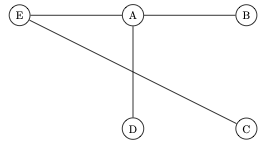
\includegraphics[keepaspectratio,alt={undirected graph}]{hw6_q2_graph.png}}
\caption{undirected graph}
\end{figure}

Formally, Members \(i\) and \(j\) are linked if either they are friends
or for some \(n \ge 1\) there are members \(a_1, a_2, \ldots, a_n\) such
that Members \(i\) and \(a_1\) are friends, Members \(a_1\) and \(a_2\)
are friends, Members \(a_2\) and \(a_3\) are friends, and so on, and
Members \(a_n\) and \(j\) are friends.

Consider a network of \(m\) members. For \(1 \le i \le m\) let \(f_i\)
be the number of friends of Member \(i\), and assume that
\(f_a \ne f_b\) for some members \(a\) and \(b\). Also assume that every
member is linked to every other member.

Let \(X_0, X_1, X_2, \ldots\) be a Markov Chain on the set of members,
with transitions based on the following proposal scheme. Given that the
chain is at Member \(i\):

\begin{itemize}
\item
  Select a friend uniformly at random from all of Member \(i\)'s
  friends.
\item
  If the selected friend is Member \(j\), then:

  \begin{itemize}
  \item
    If \(f_j \le f_i\), move to \(j\).
  \item
    If \(f_j > f_i\), toss a coin that lands heads with chance
    \(f_i / f_j\). If it lands heads, move to \(j\). If it lands tails,
    stay at \(i\).
  \end{itemize}
\end{itemize}

\textbf{a)} For states \(i \ne j\), find the one-step transition
probability \(P(i, j) = P(X_1 = j \mid X_0=i)\).

%%%% QUESTION 2a 
\begin{align*}
	P(i, j) &= P(X_1 = j \mid X_0=i) \\
	&= \begin{cases}
		1 \cdot \frac{1}{f_{i}}, \quad &\text{if $ i $ and $ j$ are friends and $ f_{j}  \le f_{i}$} \\
		\frac{f_{i}}{f_{j}} \cdot \frac{1}{f_{i}}, \quad &\text{if $ i $ and $ j $ are friends and $ f_{j} > f_{i} $ } \\
		0, \quad &\text{if $ i $ and $ j $ are not friends}
	\end{cases} \\
	&= \begin{cases}
		\frac{1}{f_{i}} & \text{if $ i $ and $ j $ are friends and $ f_{j} \le f_{i} $ }\\
		\frac{1}{f_{j}} & \text{if $ i $ and $ j $ are friends and $ f_{j} > f_{i}$} \\
		0, &\text{otherwise}
	\end{cases} \\
\end{align*}




\textbf{b)} Briefly explain why the chain has a steady state
distribution, and find that distribution. Identify it as one of the
famous ones and provide its name and parameters.


The transition matrix is symmetric by construction, because if $ i $ has more friends and is linked to $ j $ , then we propose a transition with probability $ \frac{1}{f_{i}} $, while if $ j $ has more friends and is linked to $ i $, we propose a transition with probability $ \frac{1}{f_{j}}$. Otherwise, $ P(i,j) = 0 $. Thus, the denominator is just the member that has more friends, or $ \max(f_{i}, f_{j}) $. Since $ \max(f_{i}, f_{j}) = \max(f_{j}, f_{i}) $. 

This transition matrix is also irreducible, as all Members are linked to each other (e.g BAECEADAB). 

Since we know the matrix is symmetric, and that all rows sum up to 1 due to the definition of a Markov chain, we know that the matrix is also doubly stochastic. This is because in a symmetric matrix, row $ i $ = column $ j $ if $ i=j $. We proved the previous question that a doubly stochastic transition matrix in the long run follows a uniform distribution. 

Thus, the $ X_k$ has a uniform($ \frac{1}{n} $) distribution. 


    \newpage

    \subsection{3. Bounds}\label{bounds}

A random variable \(X\), not necessarily non-negative, has \(E(X) = 20\)
and \(SD(X) = 4\). In each part below \textbf{find the best bounds you
can} based on the information given.

\textbf{a)} Find upper and lower bounds for \(P(0 < X < 40)\).

Using Chebysev's Inequality: 

\begin{align*}
	P(0<X<40) \le 1 - P(|X - \mu _{X}| \ge c) &=  1 - P(|X - \mu _{X}| \ge 20)  \\
	&= 1 - \frac{4^{2}}{20^{2}} \\
	&= 1 - \frac{1}{25} \\
	&= \frac{24}{25} \\
\end{align*}


Thus, 

\[
	\boxed{\frac{24}{25} \le P(0< X< 40) \le 1}
\]
\textbf{b)} Find upper and lower bounds for \(P(10 < X < 40)\).

We still use Chebysev's inequality, however it is two tailed. We cannot get a one tailed version. Thus, to get a lower bound, we need to look at a symmetric bound of $ P(10 < X < 30) \le P(10 < X < 40 )$ 

\begin{align*}
	P(10 < X < 30) &\ge 1- P(|X - \mu _{X}| \ge c) \\
	&= 1 - \frac{4^{2}}{10^{2}} \\
	&= \frac{21}{25} \\
\end{align*}

Our best bounds is 

\[
	\boxed{\frac{21}{25} \le P(10<X<40) \le 1}
\]


\textbf{c)} Find an upper bound for \(P(X \ge 40)\).

We cannot use Markov's Inequality because $ X $ is not nonnegative. The best bounds we could have is from Chebysev's. 

Thus we need to find $ P(X \ge 40 \cup X \le 0) = 1 - P(0<X<40) $ 

From part a, we know $ P(0<X<40) \le \frac{24}{25}$ 
\[
	\boxed{0 \le P(X\ge{40}) \le \frac{1}{25}}
\]
\textbf{d)} Find an upper bound for \(P(X^2 \ge 900)\).

For $ X^{2} $, we can now guarantee that this is a nonnegative random variable, thus we can use Markov's Inequality. 


\[
P(X \ge c) \le \frac{E[X]}{c}
\]

\[
P(X^{2} \ge 900) \le \frac{E[X^{2}]}{900}
\]
\begin{align*}
	\Var(X) &= E[X^{2}] - E[X]^{2} \\ 
	E[X^{2}] &= \Var(X) + E[X]^{2} \\	
	&= SD(X)^{2}  + E[X]^{2} \\
	&= 4^{2} + 20^{2} \\
	&= 416 \\
\end{align*}

\[
0 \le P(X^{2} \ge 900 ) \le \frac{416}{900}
\]
However, this might not be the best bound, since the squared term adds a lot of variance, and we can also partition the space to calculate Chebyshev's. 

\[
	P(X^{2} \ge 900) = P(|X| \ge 30) = P\{X \ge 30 \cup X \le -30 \}
\]

Since $ P\{X \ge 30 \cup X \le -30\} = 1 - P(-30 < X < 30) $, we can bound this function in a similar way to part  b. 

Since $ P(-30 < X < 30) \ge P(10 < X < 30) $ and $P(10 < X < 30) \ge \frac{21}{25}$ by part b. 

\[
\frac{21}{25} \le P(10 < X < 30) \le P(-30 < X < 30)
\]
From this equation, we can assert that the upper bound for $ P\{X\ge30\cup X \le -30\} \le \frac{4}{25} $ 


Thus the best bounds for $ P(X^{2} \ge 900) $ is $ \boxed{0 \le P(X^{2}\ge 900) \le \frac{4}{25}} $  
    \newpage

    \subsection*{4. Bias and Variance}\label{bias-and-variance}

Consider a probabilistic model that has a numerical parameter
\(\theta\). A ``probabilistic model'' is just a set of assumptions about
randomness. Let the random variable \(T\) be an estimator of \(\theta\).
Frequently, \(T\) is a statistic based on a random sample.

The \emph{bias} of \(T\) is defined as

\[
B_\theta (T) ~ = ~ E_\theta (T) - \theta,
\]

where the subscript \(\theta\) reminds us that \(\theta\) is the true
value of the parameter. Note that \(B_\theta(T)\) is a real-valued
function of \(\theta\), not a random variable.

Recall that \(T\) is an unbiased estimator of \(\theta\) if
\(E_\theta(T) = \theta\), that is, if \(B_\theta(T) = 0\). But in
general, estimators are biased.

The \emph{mean squared error} of the estimator \(T\) is

\[ 
MSE_\theta (T) ~ = ~ E_\theta \big( (T - \theta)^2 \big)
\]

Follow the calculation in
\href{https://data140.org/textbook/content/chapter-12/prediction-and-estimation/}{Section
12.2} of the textbook to show the \emph{bias-variance decomposition}
given by

\[
MSE_\theta (T) ~ = ~ Var_\theta(T) + B_\theta^2(T)
\]

Note that the square in the bias term makes sense. Bias has the same
units as \(T\), whereas the MSE and variance are in the square of those
units.

\begin{align*}
\MSE_{\theta}(T) &= E_{\theta}\left( (T-\theta)^{2} \right)  \\	
&= E_{\theta} \left( T^{2} - 2T\theta + \theta^{2} \right) \\
&= E_{\theta}(T^{2}) + E_{\theta}(-2T\theta) + E_{\theta}(\theta^{2}) \\
&= E_{\theta}(T^{2}) -2\theta E_{\theta}(T) + \theta^{2} \\
&= E_{\theta}(T^{2}) - E_{\theta}(T)^{2} + E_{\theta}(T)^{2} - 2\theta E_{\theta}(T) + \theta^{2} \\
&= \Var_{\theta}(T) + \theta^{2} - 2\theta E_{\theta}(T) + E_{\theta}(T)^{2} \\
&= \Var_{\theta}(T) + (E_{\theta}(T) - \theta)^{2}   \\
&= \Var_{\theta}(T) + B_{\theta}^{2}(T) \\
\end{align*}












\newpage
    \subsection*{Submission Instructions}\label{submission-instructions}

Many assignments throughout the course will have a written portion and a
code portion. Please follow the directions below to properly submit both
portions.

\subsubsection{Written Portion}\label{written-portion}

\begin{itemize}
\tightlist
\item
  Scan all the pages into a PDF. You can use any scanner or a phone
  using applications such as CamScanner. Please \textbf{DO NOT} simply
  take pictures using your phone.
\item
  Please start a new page for each question. If you have already written
  multiple questions on the same page, you can crop the image in
  CamScanner or fold your page over (the old-fashioned way). This helps
  expedite grading.
\item
  It is your responsibility to check that all the work on all the
  scanned pages is legible.
\item
  If you used \(\LaTeX\) to do the written portions, you do not need to
  do any scanning; you can just download the whole notebook as a PDF via
  LaTeX.
\end{itemize}

\subsubsection{Code Portion}\label{code-portion}

\begin{itemize}
\tightlist
\item
  Save your notebook using
  \texttt{File\ \textgreater{}\ Save\ Notebook}.
\item
  Generate a PDF file using
  \texttt{File\ \textgreater{}\ Save\ and\ Export\ Notebook\ As\ \textgreater{}\ PDF}.
  This might take a few seconds and will automatically download a PDF
  version of this notebook.

  \begin{itemize}
  \tightlist
  \item
    If you have issues, please post a follow-up on the general Homework
    6 Ed thread.
  \end{itemize}
\end{itemize}

\subsubsection{Submitting}\label{submitting}

\begin{itemize}
\tightlist
\item
  Combine the PDFs from the written and code portions into one PDF.
  \href{https://smallpdf.com/merge-pdf}{Here} is a useful tool for doing
  so.
\item
  Submit the assignment to Homework 6 on Gradescope.
\item
  \textbf{Make sure to assign each page of your pdf to the correct
  question.}
\item
  \textbf{It is your responsibility to verify that all of your work
  shows up in your final PDF submission.}
\end{itemize}

If you are having difficulties scanning, uploading, or submitting your
work, please read the
\href{https://edstem.org/us/courses/94054/discussion/7533569}{Ed Thread}
on this topic and post a follow-up on the general Homework 6 Ed thread.

    \subsection{\texorpdfstring{\textbf{We will not grade assignments which
do not have pages selected for each
question.}}{We will not grade assignments which do not have pages selected for each question.}}\label{we-will-not-grade-assignments-which-do-not-have-pages-selected-for-each-question.}

    \begin{tcolorbox}[breakable, size=fbox, boxrule=1pt, pad at break*=1mm,colback=cellbackground, colframe=cellborder]
\prompt{In}{incolor}{ }{\boxspacing}
\begin{Verbatim}[commandchars=\\\{\}]

\end{Verbatim}
\end{tcolorbox}


    % Add a bibliography block to the postdoc
    
    
    
\end{document}
